\section{Experimental Setup}
The objective of the experiment was to collect timing performance data for resolving DNS queries over chosen protocols and ultimately compare them to the experimental performance of DNS-over-HTTP/3.  In order to analyze performance between DNS-over-HTTP/3 and other various protocols, a software package was built to make the appropriate timing measurements for http/3, http/2, http/1.1, http/1.0, tls1.3, tls1.2, tls1.0, and traditional dns. The measurements were evaluated for Google and Cloudflare DNS servers, as both support the http/3 protocol for resolving dns queries [7,8].  The software package included industry standard tools, with curl being the most important to support all the protocols mentioned above. In order to fully support experimental http/3, curl was built from source and had to have an implementation of a QUIC transport protocol, and in this case, Quiche was the implementation that was chosen \cite{curl,quiche}.  To get samples for traditional DNS, kdig was the tool selected [3].  A build script was used to install package dependencies, clone the required repos, and build the tools that were needed for this experiment. At the end of the build script, a cronjob was initialized to run the data collection script every 15 minutes over the course of an entire week, with the experiment being completed at the end of that time period.  The data collection script would perform the curl, kdig, ping, and traceroute commands and pipe the output into respective text files. The commands resolved Amazon’s URL and collected timing data for name lookup, connection, app connection, pre-transfer, redirect, start transfer, and time total [6].  Once the experiment was completed, a cleanup script would run that would uninstall any packages the build script had to install, as well as remove the built software tools and remove the cronjob. 
Initially, the software package was sent to volunteers to run on their personal machines. The only requirement for users to be able to run the software package was to have a machine with a distribution of Linux or Mac operating systems. Only a few participants could be sourced to run the experiment and they all resided in the same county in North Alabama. This gave data for a small geographical area and did not add depth to the data as there was no variation in networks or locations. As a next step to broaden our data collection vantage points, Google Compute Engine virtual machines were utilized [4].  Since the virtual machines are a part of a well constructed computing network, the addition of Linux traffic shaping was added to the experiment setup to simulate three types of network: a high-grade, mid-grade, and low-grade network defined in Table 1.  Three virtual machines were instantiated in each region that Google Compute Engine offered (one for each type of network) and the experiment was run on each for data collection; the regions are shown in Figure A.
\begin{figure}[htpb]
    \centering
    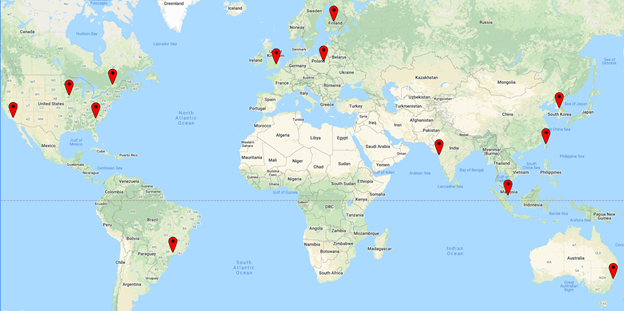
\includegraphics[width=8cm]{figures_and_tables/map.png}
    \caption{Fig. A. The locations for the virtual machines: California, Iowa, South Carolina, Canada, Brazil, England, Poland, Finland, India, Singapore, Taiwan, South Korea, Australia [5]}
    \label{fig:map}
\end{figure}